\section{Results}\label{sec:results}

\subsection{Base case}
As a reference for all following calculations, a model representing the Blennerhassett Island Bridge's final design is investigated. The results obtained by the analysis are then compared to the ones in the design drawings for plausibility. A particular challenge is the determination of the self-equilibrium stress state. As the arch was defined as an unsuitable parabola, appropriate hanger forces were determined by trial and error in the design. These permanent hanger forces of the final design are available in the drawings. However, they are unsuitable for calculating the base case, as the load distribution in the model is simplified. Instead of another trial and error procedure for the base case, the hanger forces are obtained as the result of a simultaneous arch and tie moment optimisation. Thereby, the arch's moment is weighed by a factor of 1.5 to achieve an optimal similarity. Further, the hanger forces are bounded between 25\% and 45\% of their nominal strength. The base case's internal force distributions for the permanent state are shown in Fig. \ref{fig:base_case_permanent}. Instead of the normal force in the hangers, the demand over capacity ratio is shown directly. Only the hangers of one set are shown, namely the ones inclined to the right side, and the dots are connected for readability. As a comparison, the extreme values found on the design drawings are also shown.

\begin{figure}[H]
    \centering
    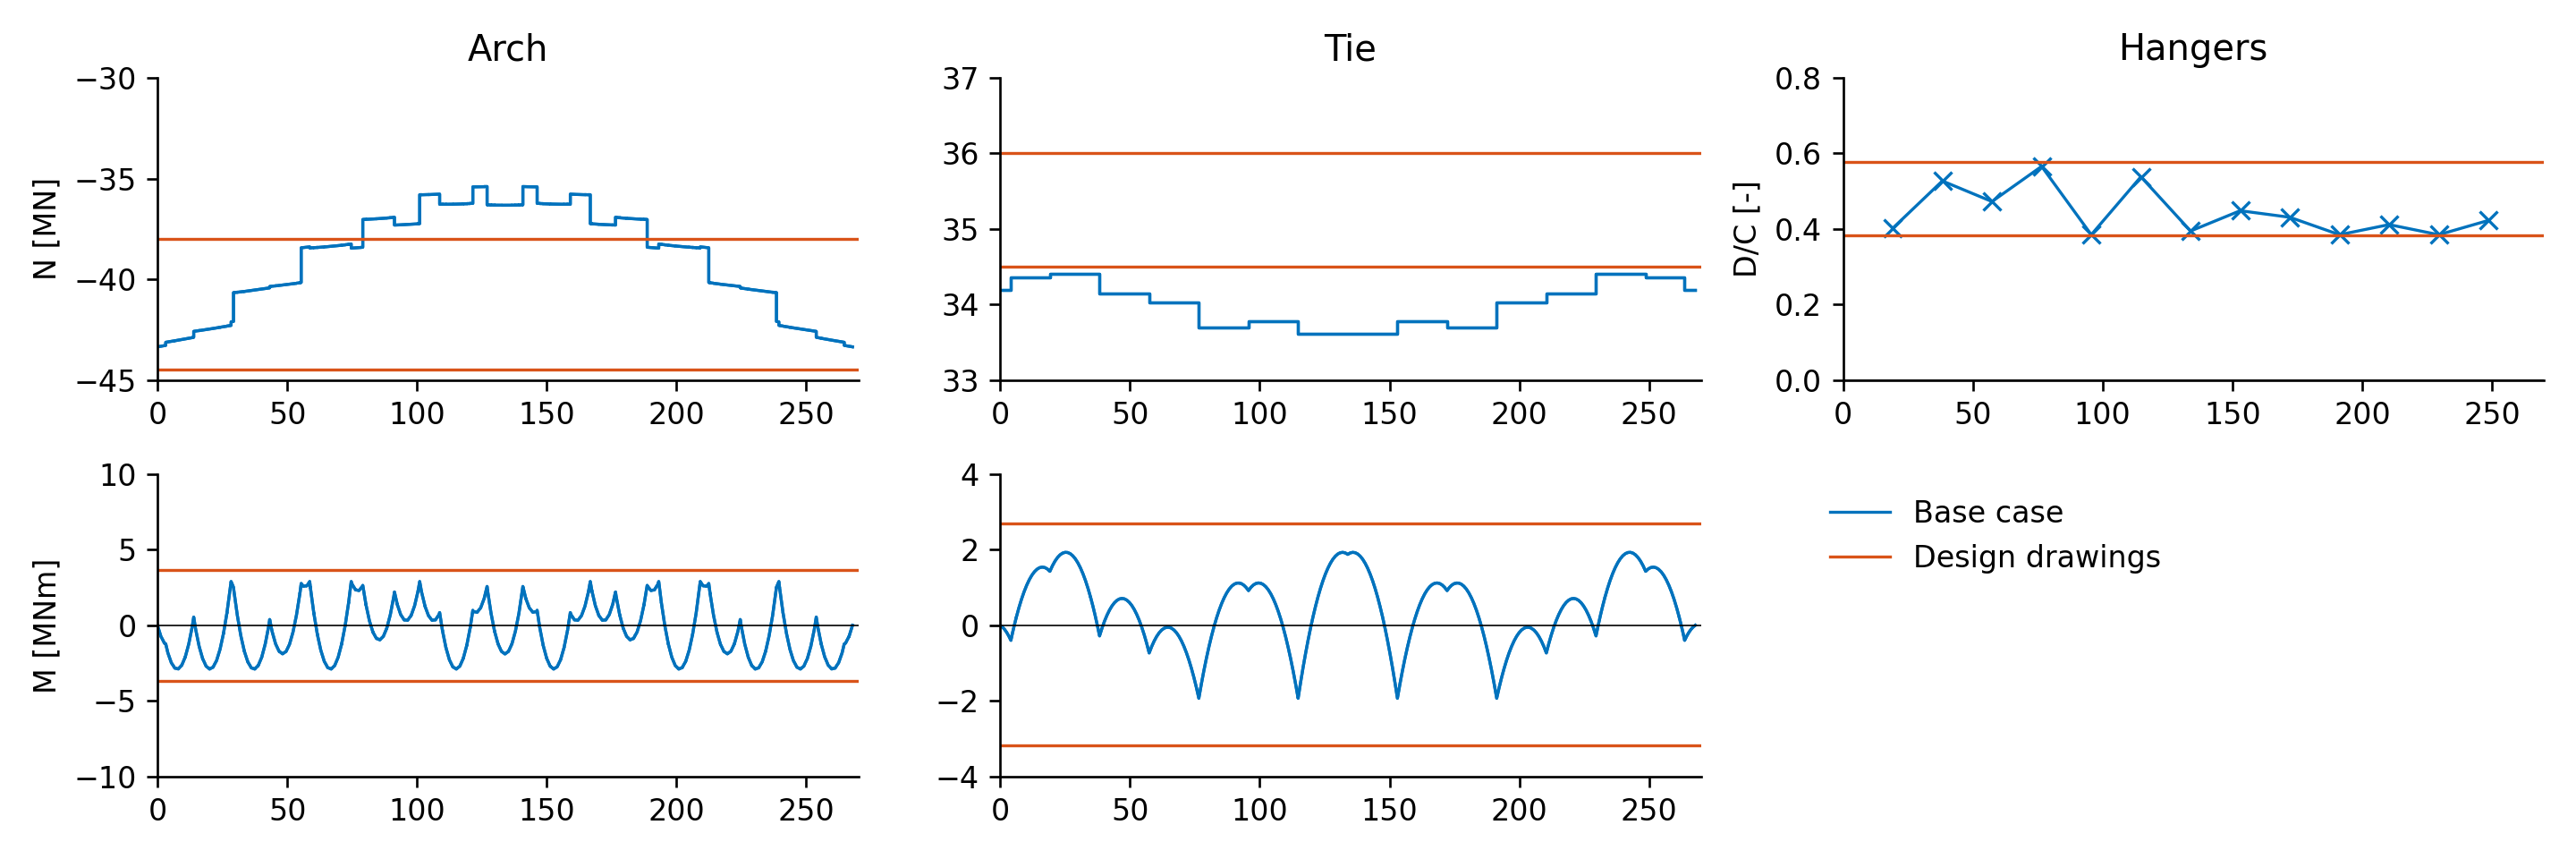
\includegraphics[width=\textwidth]{calculations/Base case/Permanent state.png}
    \caption{Permanent internal forces of the base case and reference values from the drawings}
    \label{fig:base_case_permanent}
\end{figure}

It can be seen that the moment distributions in the arch and the tie, as well as the normal forces in the hangers, match the design drawings very well. Only for the normal force in the arch rib and the tie girder an offset of \SI{2}{MN} can be observed. This difference is probably due to underestimating the weight of the bridge and its simplified assignment to the beams. However, overall the obtained internal force distribution matches the design drawings sufficiently well. It can be concluded, that for a fixed arch shape the simultaneous arch and tie moment optimisation yields adequate results.\medskip

Another comparison is drawn between the effects under characteristic live loads. As there are countless live load combinations, which are to be accounted for, it makes sense to look at the entire ranges of possible internal forces. They are shown in Fig. \ref{fig:base_case_live} by the two blue lines representing the lower and the upper limit. They are compared to the extreme values found in the design drawings.

\begin{figure}[H]
    \centering
    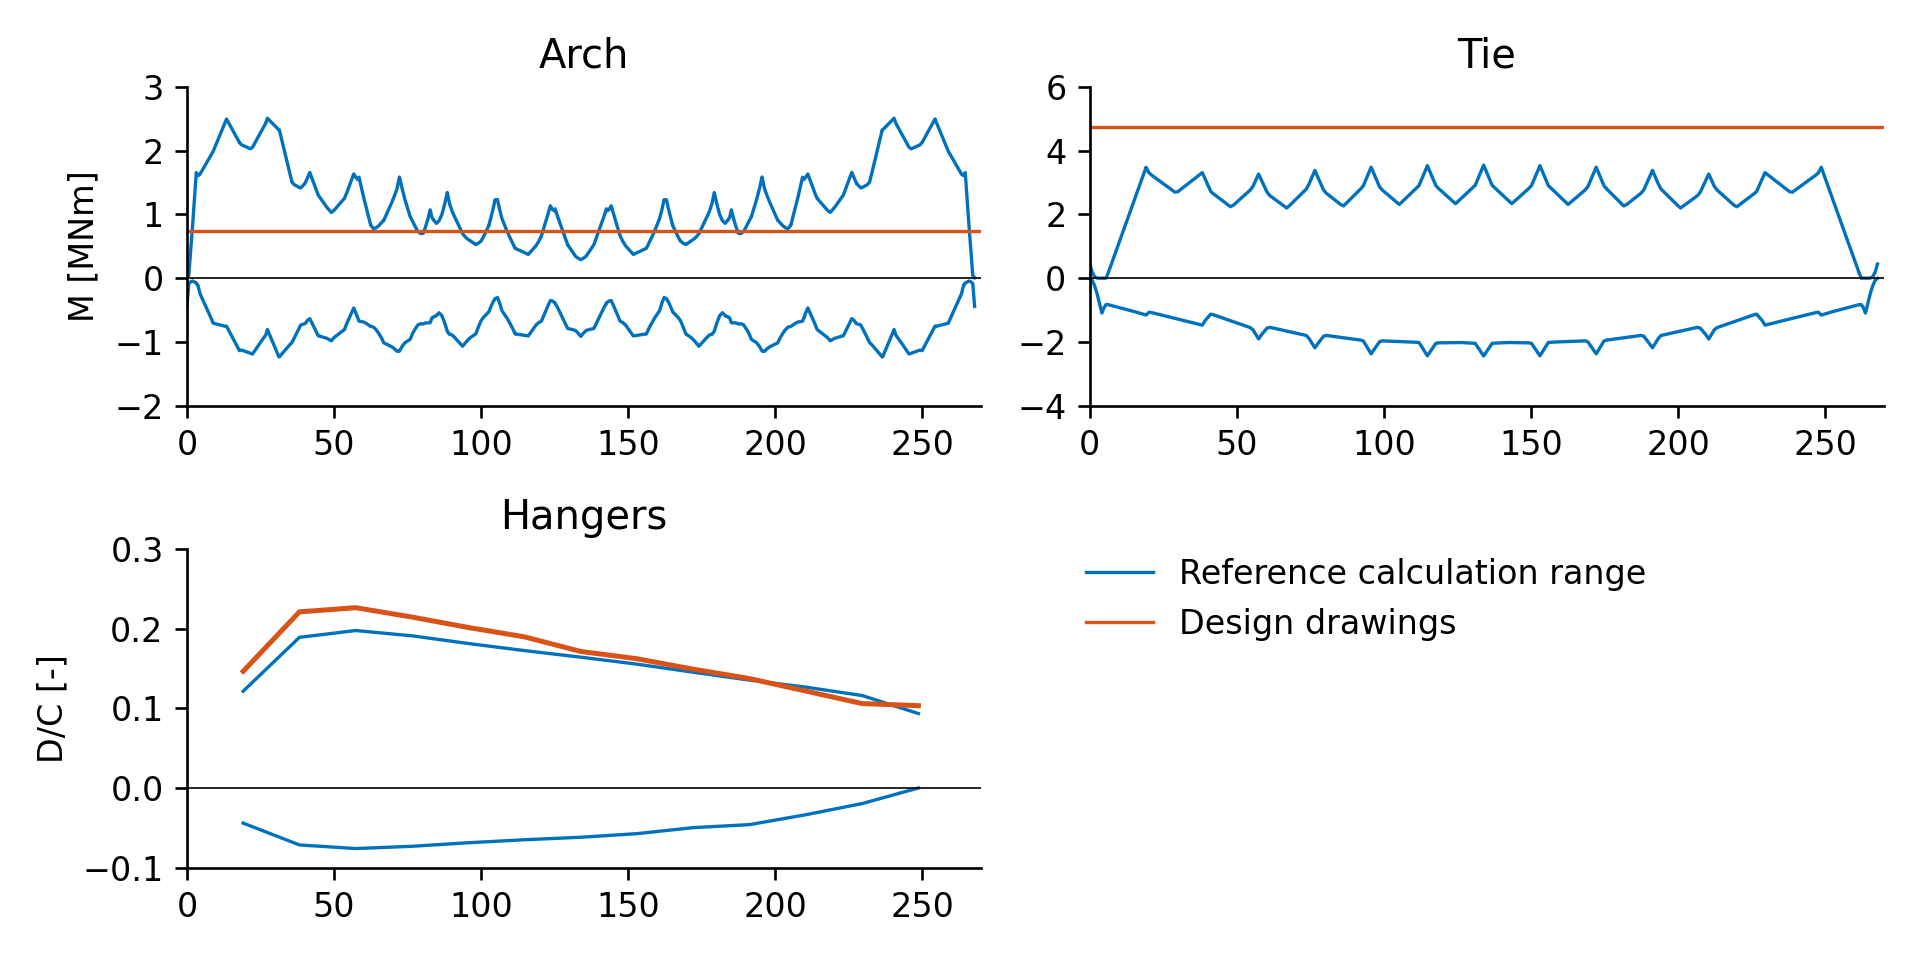
\includegraphics[width=0.8\textwidth]{calculations/Base case/Live load.png}
    \caption{Range of internal forces effects under live loading}
    \label{fig:base_case_live}
\end{figure}

The moments in the arch given in the design drawings do not correspond to the maximum for the considered load case. The considerable difference cannot be explained in another way and seems physically impossible. The moment distribution in the tie and the hangers' normal forces seem to agree on the other hand. Apparently, the live loading is only slightly overestimated in the model, which can be seen particularly well in the hangers' demand over capacity ratios. These differences are accepted, as it is not the goal of this Thesis to reproduce the results from the design drawings. Interestingly, in particular, the arch segment near the knuckle is affected by strong bending moments. On the other hand, in the tie girder, the range of effects under live loading is well distributed. Apparently, the influence lines for the moments in the tie girder at the different cross-girders follow the same shape. For the hangers, it is the second one from the knuckle connected toward the middle of the arch that undergoes the largest normal force. Towards the other side of the hangers set, the hanger forces decrease. The stronger affected hangers have in common that their inclination is closer to the arch's inclination at their respective connection node. The arch is very stiff on axial loading and comparably weaker on perpendicular forces. Therefore, at the arch nodes, smaller displacements in the hanger's direction are expected for the strongly affected hangers, explaining their higher normal forces. Only the first hanger does not follow this rule, which can be explained by its smaller area of influence. \medskip

\newpage
\subsection{Arch shape}
Traditionally, mainly the circle and the parabola have been used as arch shapes. The parabola has served well as a shape for traditional tied-arch bridges with vertical hangers. In this case, the vertical hanger forces on the arch are evenly distributed and the respective thrust line matches the parabola. For network tied-arch bridges, circular shapes have been considered suitable for radial arrangements. In this case, uniform hanger forces cause an approximately radial loading on the arch, which results in a circular thrust line. For a rise to span ratio of 0.2, the two shapes diverge by at most 0.8\% of the span. While this differences might seem negligible on a drawing, the impact of this difference on the arch's moment distribution is significant, as it is bigger than its usual cross-section height. In this section, the arch shape is first investigated individually as it impacts the investigation of all other variables. \medskip

Multiple approaches to determine the arch shape have been introduced in Section \ref{sec:met_arch}. All of them are linked to the thrust line, which is approximately the most efficient shape. The following four arch shapes are compared in this investigation.
\begin{enumerate}
    \item Thrust line: This shape is obtained numerically as the thrust line for the hanger forces obtained from a tie moment optimisation. The respective hanger forces are uniform at $N_p=\SI{2.4}{MN}$ which corresponds to 45\% of their characteristic resistance.
    \item Polynomial thrust line approximation: The above thrust line is approximated by a quartic function. The quartic function is described by Eq. \eqref{eq:polynomial_shape} and the shape parameter $b$. This parameter is obtained by a least squares approximation. It fulfills the conditions $y(0)=r$ and $y(s/2)=0$
    \begin{equation}
        y(x)=r \cdot \left(1 - b \cdot \left(\frac{2\,x}{s}\right)^2 - (1-b) \left(\frac{2\,x}{s}\right)^4 \right)
        \label{eq:polynomial_shape}
    \end{equation}
    \item Spline thrust line approximation: As a second approximation of the thrust line a cubic spline defined by the arch-hanger connection nodes is used. These nodes are therefore represented at their exact location.
    \item Thrust line of continuous hanger arrangement: This shape is the thrust line of the hypothetical continuous hanger arrangement, which was introduced in Section [].
\end{enumerate}

These shapes are hardly distinguishable by eye. To make their differences visible, only their respective deviations to the parabolic shape are shown in Fig. \ref{fig:arch_shapes_13}. Also a circular arch is shown to put the results into perspective.

\begin{figure}[H]
    \centering
    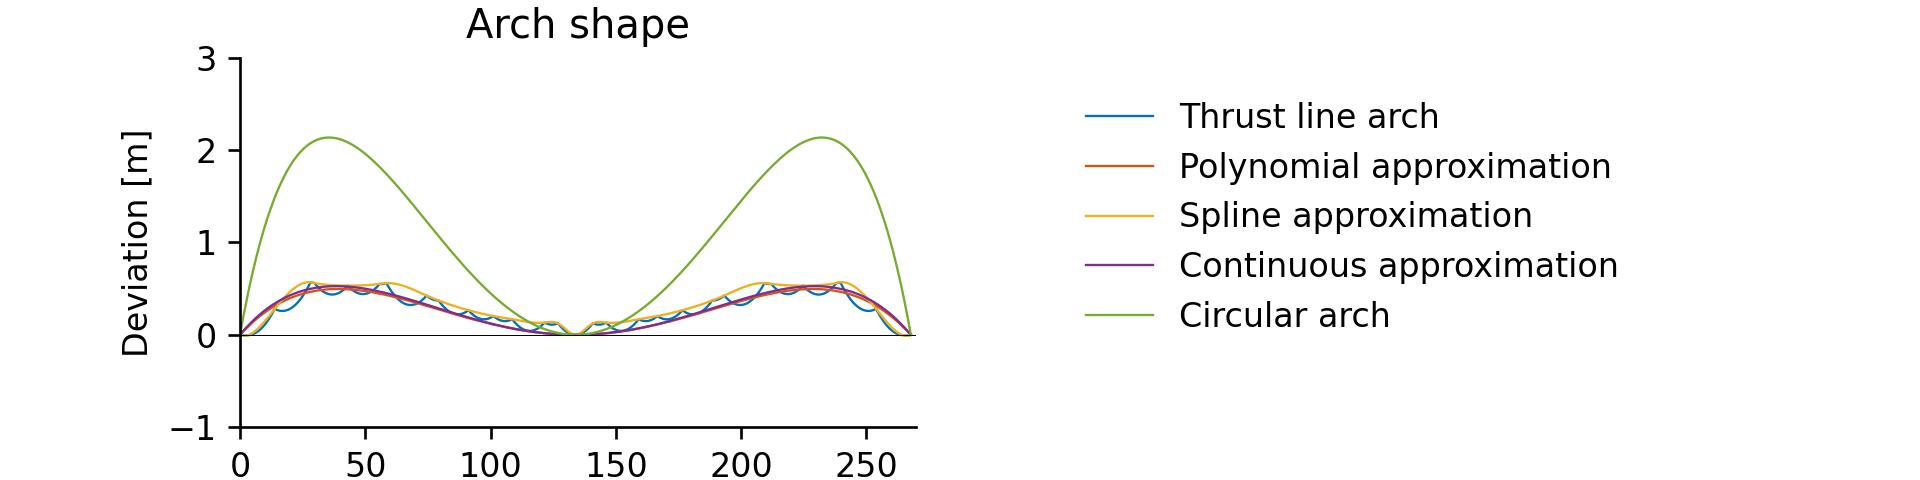
\includegraphics[trim={0 0 2cm 0},clip, width=0.8\textwidth]{calculations/arch shape/arch_shapes_13.png}
    \caption{Deviation of arch shapes from parabolic shape}
    \label{fig:arch_shapes_13}
\end{figure}

In the range between the circular and the parabolic shape, the thrust line tends slightly to the parabolic side. From the similarity between the polynomial and the continuous approximation, it can be concluded, that if the hanger arrangement is dense enough, a quartic function can yield an appropriate arch shape for this hanger arrangement pattern. All three approximations seem to fit the thrust line reasonably well. But to investigate the impacts of the remain deviations from the thrust line, the corresponding permanent moment distribution is presented in Fig. \ref{fig:arch_permanent_moments_13}.

\begin{figure}[H]
    \centering
    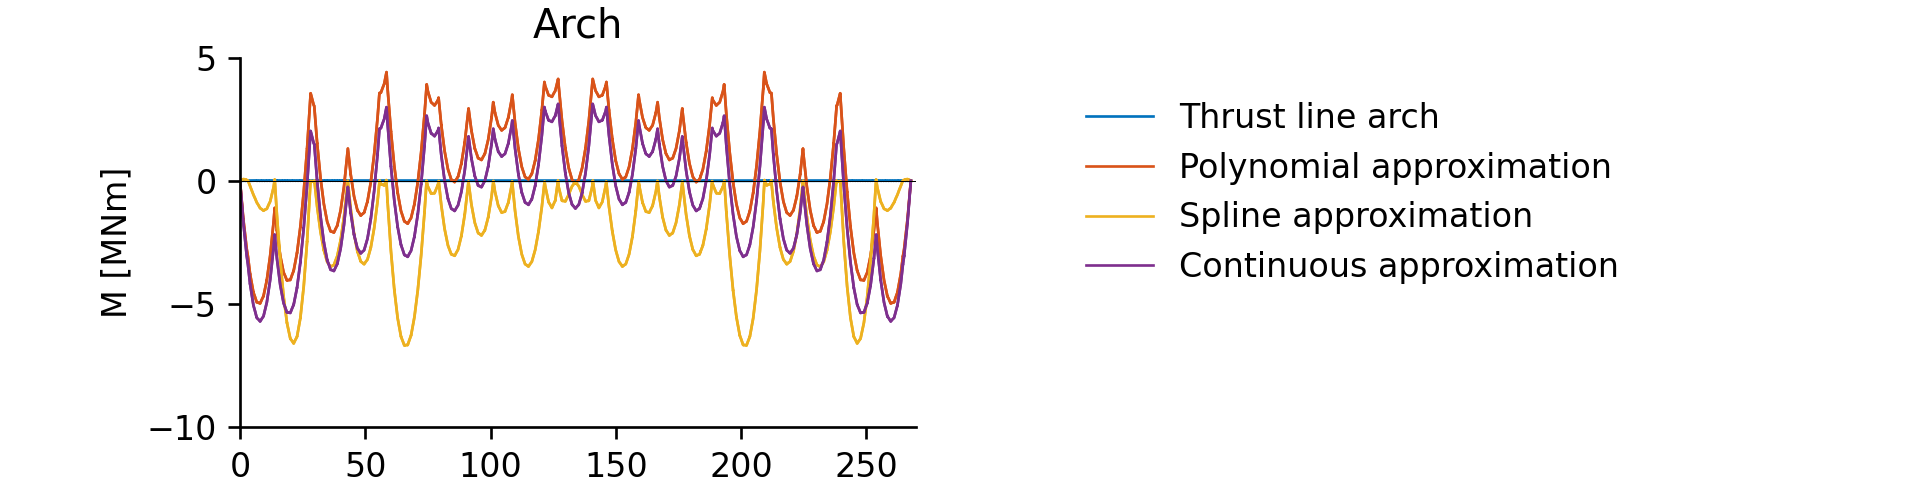
\includegraphics[trim={0 0 2cm 0},clip, width=0.8\textwidth]{calculations/arch shape/permanent state_13.png}
    \caption{Permanent arch moment distributions depending on arch shape}
    \label{fig:arch_permanent_moments_13}
\end{figure}

Despite the apparent match of the arch shapes, significant bending moments result in each of the three approximations. The spline approximation's moment distribution is strictly negative, which relies on the characteristic that a spline lies above the approximately linear thrust line and only matches it at the connection nodes. It is particularly interesting, that all approximations feature a similar parabolic moment distribution between the arch-hanger connection nodes. While these moment distributions resulting for the approximated shapes are certainly considerable, it is practically infeasible to find a simple shape matching the arch thrust line. Any shape with an approximately constant radius $R$ results in a certain deviation from the thrust line and the corresponding moment deviation $\Delta M$. This deviation can be approximated depending on the distance between two hanger points $d$ and the arch's normal force $N$ according to Eq. \eqref{eq:moment_deviation}.

\begin{equation}
    \Delta M=-\left(R-\sqrt{R^2-\left(d/2\right)^2}\right) \cdot N
    \label{eq:moment_deviation}
\end{equation}

For the Blennerhassett Island Bridge, these variables roughly correspond to $R=\SI{194}{m}$, $d=\SI{17}{m}$ and $N=\SI{40}{MN}$. Eq. \eqref{eq:moment_deviation} yields a moment deviation of $\Delta M=\SI{7.5}{MNm}$ coming close to the value observed in Fig. \ref{fig:arch_shapes_13}. From the analytical form of Eq. \eqref{eq:moment_deviation} it can further be concluded, that a reduction of the hanger node spacing has a more than proportional impact on the bending moment deviation. To put these deviations into the context of the design verifications, the demand over capacity ratios resulting in the arch are shown in Table \ref{tab:arch_shape_dc_13} for each approach.

\begin{table}[H]
    \centering
    \input{calculations/arch shape/dc_comparison_13.txt}
    \caption{Arch design verifications considering different shapes}
    \label{tab:arch_shape_dc_13}
\end{table}














\subsection{Hanger density}
It is evident, that an increase of the amount of hangers, can yield a substantial benefit by reducing the decisive effects in the extreme event of cable loss. For the design of the Blennerhassett Island Bridge, a detailed dynamic analysis was conducted, which allowed to reduce the dynamic amplification factor down to 1.6. Nevertheless, the extreme event of cable loss was decisive for the arch segments.

\subsection{Floor beam density}
